% Diagram Kelas - Sistem Informasi Usaha Bagan
% Dibuat dengan TikZ (shapes.multipart), kertas A3 landscape.
% Mencerminkan model Django yang AKTIF di aplikasi web.
\documentclass[11pt]{article}
\usepackage[a3paper,landscape,margin=1cm]{geometry}
\usepackage[T1]{fontenc}
\usepackage[utf8]{inputenc}
\usepackage{tikz}
\usepackage{adjustbox}
\usetikzlibrary{arrows.meta,calc,shapes.multipart,positioning}
\pagestyle{empty}

\tikzset{
  % kotak entitas: 2 bagian (nama | atribut)
  entity/.style={draw=blue!55!black, rectangle split, rectangle split parts=2,
                 font=\scriptsize, align=left, fill=blue!4, inner sep=3pt,
                 rectangle split draw splits=true},
  % kotak entitas: 3 bagian (nama | atribut | method)
  entity3/.style={draw=blue!55!black, rectangle split, rectangle split parts=3,
                  font=\scriptsize, align=left, fill=blue!6, inner sep=3pt},
  % relasi
  assoc/.style={thick, black!65},
  comp/.style={thick, black!65, {Diamond[fill=black!70,length=5pt,width=3.6pt]}-},
  mult/.style={font=\scriptsize, black!55, inner sep=1pt},
}

\begin{document}
\begin{adjustbox}{max width=\textwidth, max totalheight=\textheight, center}
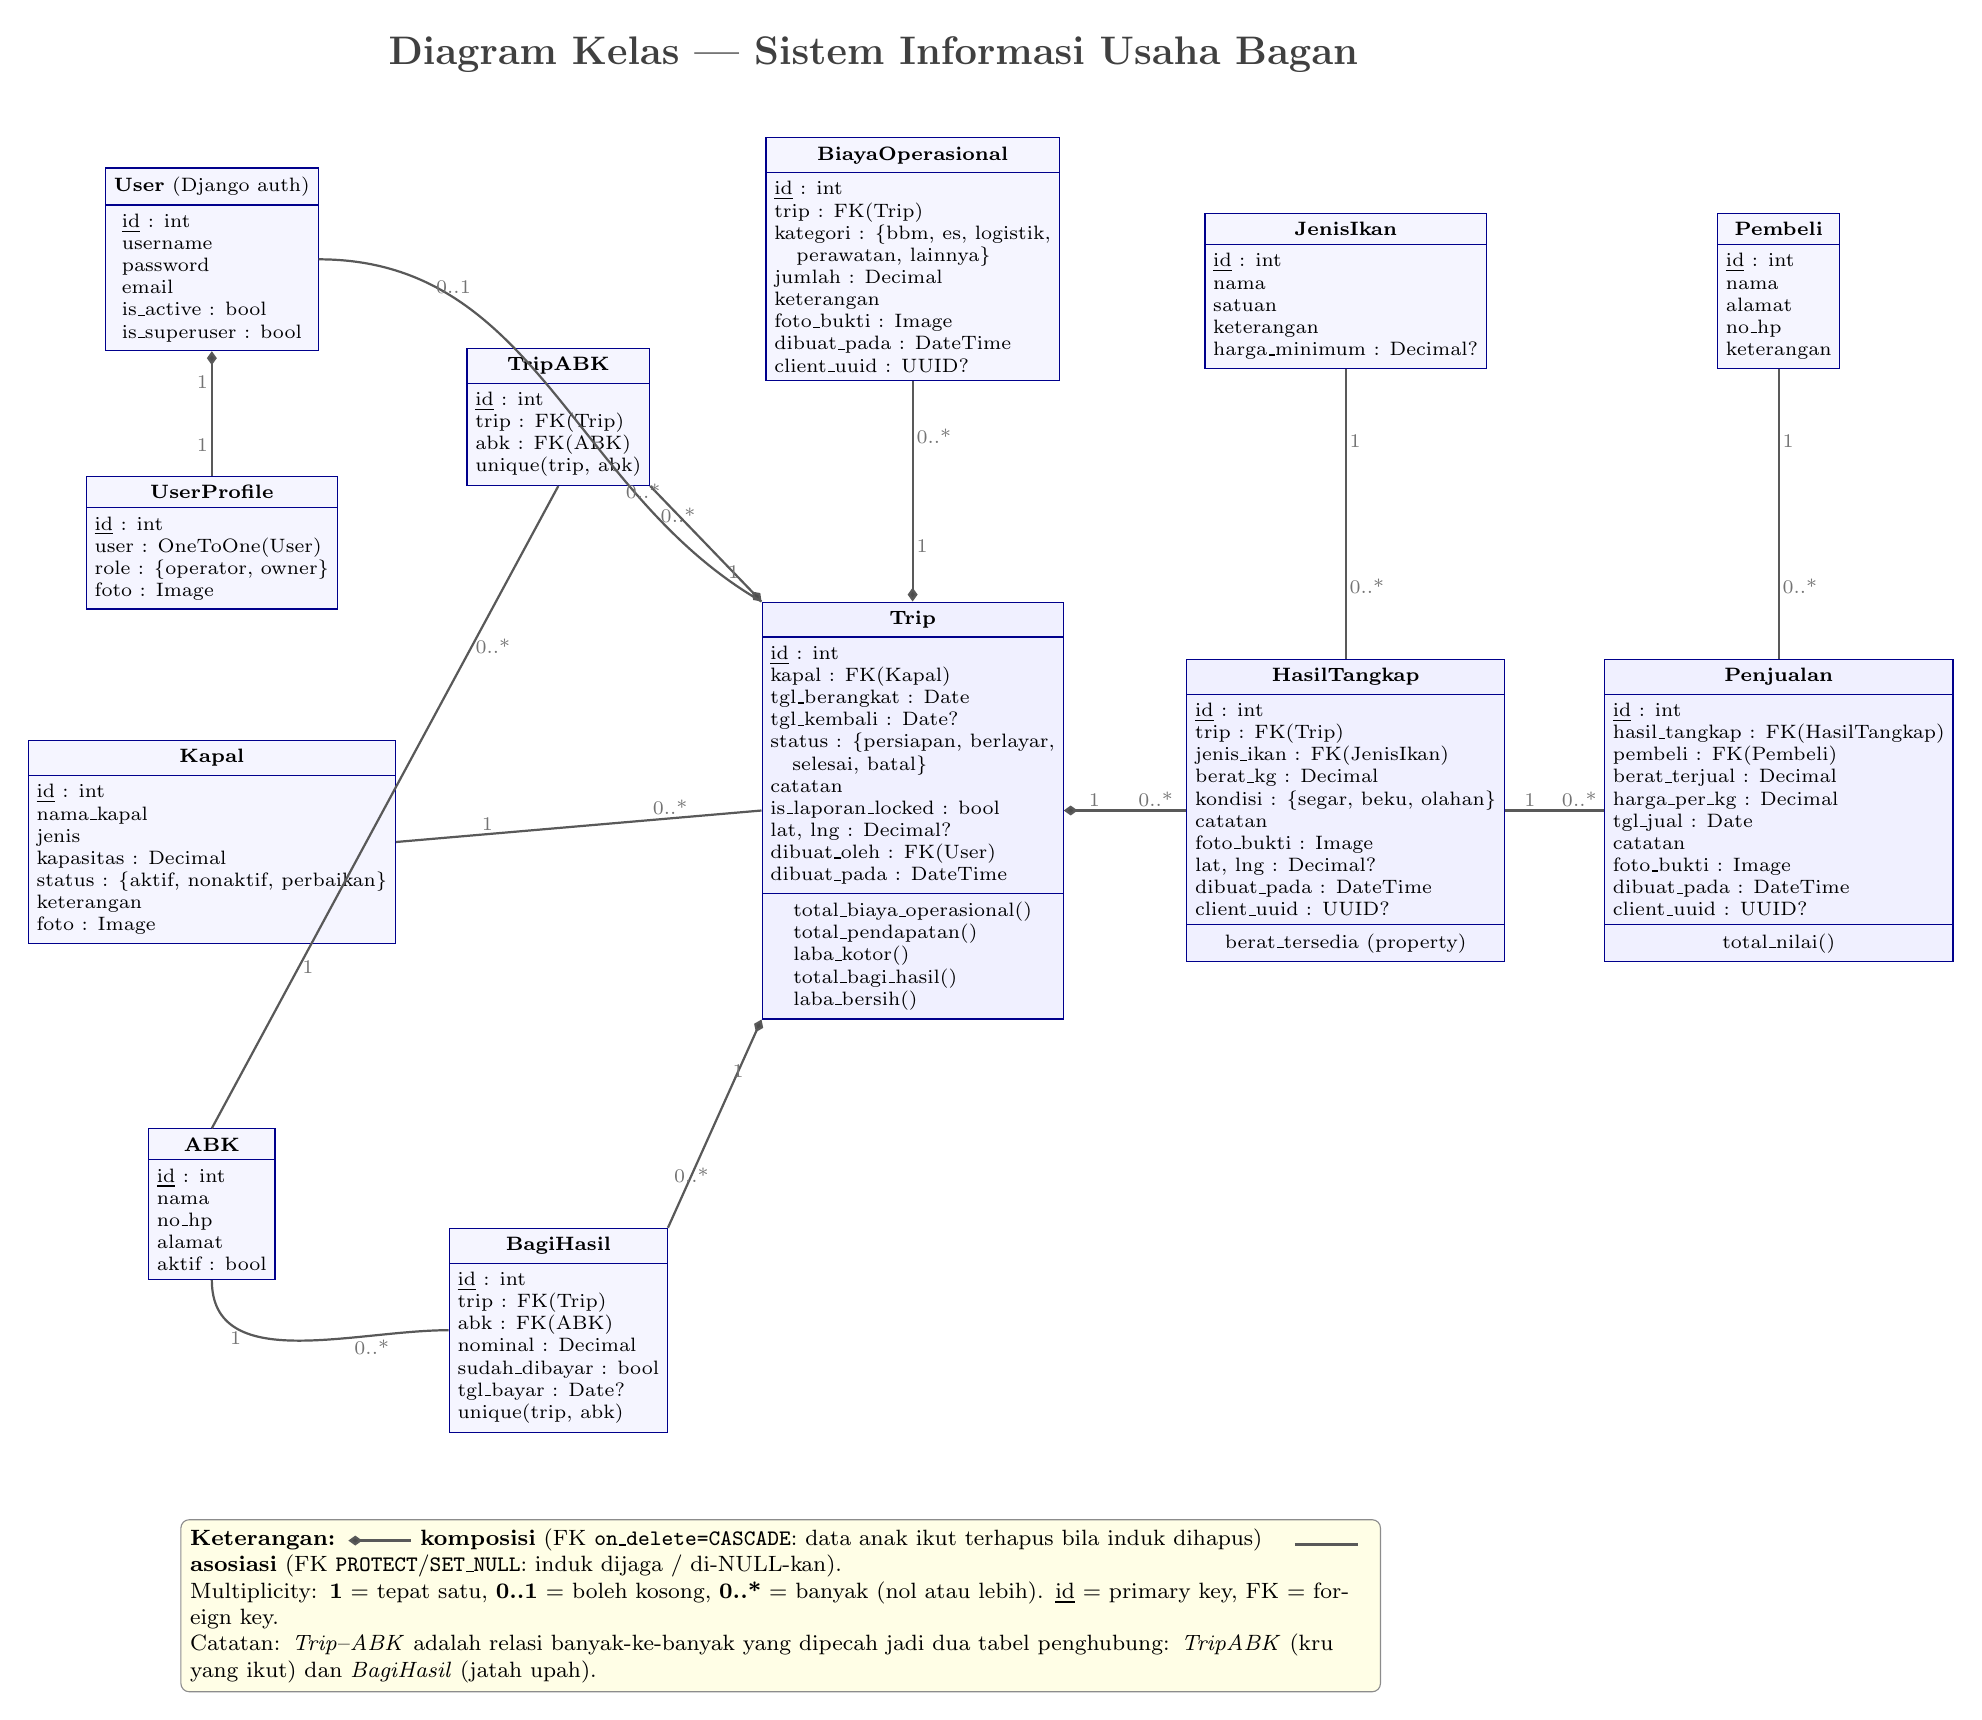
\begin{tikzpicture}[every node/.style={transform shape}]

\node[font=\Large\bfseries, black!75] at (10,15.6) {Diagram Kelas — Sistem Informasi Usaha Bagan};

% =================== KELAS / ENTITAS ===================
\node[entity] (user) at (1.6,13) {\textbf{User} \scriptsize(Django auth)
  \nodepart{two}\underline{id} : int\\ username\\ password\\ email\\ is\_active : bool\\ is\_superuser : bool};

\node[entity] (profile) at (1.6,9.4) {\textbf{UserProfile}
  \nodepart{two}\underline{id} : int\\ user : OneToOne(User)\\ role : \{operator, owner\}\\ foto : Image};

\node[entity] (kapal) at (1.6,5.6) {\textbf{Kapal}
  \nodepart{two}\underline{id} : int\\ nama\_kapal\\ jenis\\ kapasitas : Decimal\\ status : \{aktif, nonaktif, perbaikan\}\\ keterangan\\ foto : Image};

\node[entity] (abk) at (1.6,1.0) {\textbf{ABK}
  \nodepart{two}\underline{id} : int\\ nama\\ no\_hp\\ alamat\\ aktif : bool};

\node[entity] (tripabk) at (6.0,11.0) {\textbf{TripABK}
  \nodepart{two}\underline{id} : int\\ trip : FK(Trip)\\ abk : FK(ABK)\\ \scriptsize unique(trip, abk)};

\node[entity] (bagihasil) at (6.0,-0.6) {\textbf{BagiHasil}
  \nodepart{two}\underline{id} : int\\ trip : FK(Trip)\\ abk : FK(ABK)\\ nominal : Decimal\\ sudah\_dibayar : bool\\ tgl\_bayar : Date?\\ \scriptsize unique(trip, abk)};

\node[entity3] (trip) at (10.5,6) {\textbf{Trip}
  \nodepart{two}\underline{id} : int\\ kapal : FK(Kapal)\\ tgl\_berangkat : Date\\ tgl\_kembali : Date?\\ status : \{persiapan, berlayar,\\ \hspace{1em}selesai, batal\}\\ catatan\\ is\_laporan\_locked : bool\\ lat, lng : Decimal?\\ dibuat\_oleh : FK(User)\\ dibuat\_pada : DateTime
  \nodepart{three}total\_biaya\_operasional()\\ total\_pendapatan()\\ laba\_kotor()\\ total\_bagi\_hasil()\\ laba\_bersih()};

\node[entity] (biaya) at (10.5,13) {\textbf{BiayaOperasional}
  \nodepart{two}\underline{id} : int\\ trip : FK(Trip)\\ kategori : \{bbm, es, logistik,\\ \hspace{1em}perawatan, lainnya\}\\ jumlah : Decimal\\ keterangan\\ foto\_bukti : Image\\ dibuat\_pada : DateTime\\ client\_uuid : UUID?};

\node[entity3] (tangkap) at (16,6) {\textbf{HasilTangkap}
  \nodepart{two}\underline{id} : int\\ trip : FK(Trip)\\ jenis\_ikan : FK(JenisIkan)\\ berat\_kg : Decimal\\ kondisi : \{segar, beku, olahan\}\\ catatan\\ foto\_bukti : Image\\ lat, lng : Decimal?\\ dibuat\_pada : DateTime\\ client\_uuid : UUID?
  \nodepart{three}berat\_tersedia \scriptsize(property)};

\node[entity] (jenisikan) at (16,12.6) {\textbf{JenisIkan}
  \nodepart{two}\underline{id} : int\\ nama\\ satuan\\ keterangan\\ harga\_minimum : Decimal?};

\node[entity3] (penjualan) at (21.5,6) {\textbf{Penjualan}
  \nodepart{two}\underline{id} : int\\ hasil\_tangkap : FK(HasilTangkap)\\ pembeli : FK(Pembeli)\\ berat\_terjual : Decimal\\ harga\_per\_kg : Decimal\\ tgl\_jual : Date\\ catatan\\ foto\_bukti : Image\\ dibuat\_pada : DateTime\\ client\_uuid : UUID?
  \nodepart{three}total\_nilai()};

\node[entity] (pembeli) at (21.5,12.6) {\textbf{Pembeli}
  \nodepart{two}\underline{id} : int\\ nama\\ alamat\\ no\_hp\\ keterangan};

% =================== RELASI ===================
% Komposisi (on_delete=CASCADE): hidup-mati anak ikut induk -> wajik penuh di sisi induk
\draw[comp] (user.south) -- node[mult,near start,left]{1} node[mult,near end,left]{1} (profile.north);
\draw[comp] (trip.north west) -- node[mult,near start]{1} node[mult,near end]{0..*} (tripabk.south east);
\draw[comp] (trip.south west) -- node[mult,near start]{1} node[mult,near end]{0..*} (bagihasil.north east);
\draw[comp] (trip.north) -- node[mult,near start,right]{1} node[mult,near end,right]{0..*} (biaya.south);
\draw[comp] (trip.east) -- node[mult,near start,above]{1} node[mult,near end,above]{0..*} (tangkap.west);

% Asosiasi (on_delete=PROTECT / SET_NULL): induk tidak boleh terhapus (atau jadi NULL)
\draw[assoc] (kapal.east) -- node[mult,near start,above]{1} node[mult,near end,above]{0..*} (trip.west);
\draw[assoc] (user.east) to[out=0,in=150] node[mult,near end,above]{0..*} node[mult,near start,above]{0..1} (trip.north west);
\draw[assoc] (abk.north) -- node[mult,near start,right]{1} node[mult,near end,right]{0..*} (tripabk.south);
\draw[assoc] (abk.south) to[out=-90,in=180] node[mult,near start,below]{1} node[mult,near end,below]{0..*} (bagihasil.west);
\draw[assoc] (jenisikan.south) -- node[mult,near start,right]{1} node[mult,near end,right]{0..*} (tangkap.north);
\draw[assoc] (tangkap.east) -- node[mult,near start,above]{1} node[mult,near end,above]{0..*} (penjualan.west);
\draw[assoc] (pembeli.south) -- node[mult,near start,right]{1} node[mult,near end,right]{0..*} (penjualan.north);

% =================== LEGENDA ===================
\node[draw=black!45, rounded corners=3pt, align=left, font=\footnotesize,
      fill=yellow!10, text width=15cm, anchor=north west] at (1.2,-3.0)
  {\textbf{Keterangan:}
   \tikz\draw[comp](0,0)--(0.8,0); \textbf{komposisi} (FK \texttt{on\_delete=CASCADE}: data anak ikut terhapus bila induk dihapus) \quad
   \tikz\draw[assoc](0,0)--(0.8,0); \textbf{asosiasi} (FK \texttt{PROTECT}/\texttt{SET\_NULL}: induk dijaga / di-NULL-kan).\\
   Multiplicity: \textbf{1} = tepat satu, \textbf{0..1} = boleh kosong, \textbf{0..*} = banyak (nol atau lebih). \underline{id} = primary key, FK = foreign key.\\
   Catatan: \emph{Trip}–\emph{ABK} adalah relasi banyak-ke-banyak yang dipecah jadi dua tabel penghubung: \emph{TripABK} (kru yang ikut) dan \emph{BagiHasil} (jatah upah).};

\end{tikzpicture}%
\end{adjustbox}
\end{document}
